\chapter{Proposed Solution}
\label{chap:ProposedSolution}

This chapter contains a detailed description of the final solution: data preparation, approaches taken to implement the n-gram sorters, and various engineering details.

\section{Solution Overview}
\label{sec:ProposedSolution-Overview}
The objective of this implementation is the following: suggest the most likely tokens at every step of the completion process. The main idea is to leave the existing, AST-based code completion engine in place, and just enhance the sorting strategy. For this, I implemented two separate sorters based on n-gram models. That means that after the list of completion candidates is proposed, it gets sorted based on each n-gram's probability, so that the most relevant completions are shown first.

The n-gram models implemented were the unigram and the bigram. N-gram models of a higher order, such as 3- and 4-gram models, were not considered due their computational complexity: the frequency table increases exponentially with every new order of \textit{n} which makes the calculation of probabilities too slow for the task, where results must be updated at every keystroke.

\subsection{Unigram Sorting}
The first implementation, unigram-based sorting, is based on the 1-gram analysis, which means that we only take into consideration the actual token being completed. The implementation of the unigram model itself comes down to calculating individual token frequencies, i.e. the number of occurrences of each token in the source code. Then the completion candidates are sorted according to each one's frequency. In Listings \ref{lst:unigramCode1}, \ref{lst:unigramCode2} and \ref{lst:unigramCode3}  you can see the frequencies data being passed to the sorter, and then the completions being sorted based on that information:

\begin{lstlisting}[caption={The unigram sorter implementation: passing the frequencies to the sorter}, label={lst:unigramCode1}]
    FrequencyCompletionSorter >> initialize
        sorter := FrequencySorter new.
        sorter frequencies: Unigram uniqueInstance frequencies
\end{lstlisting}

\begin{lstlisting}[caption={The sorter implementation: sorting the candidates according to their frequencies}, label={lst:unigramCode2}]
    FrequencySorter >> sort: anOrderedCollection
        ^ anOrderedCollection sort: [ :a :b |
            (frequencies at: a contents ifAbsent: 0) >
                (frequencies at: b contents ifAbsent: 0) ]
\end{lstlisting}

\begin{lstlisting}[caption={The unigram sorter implementation: returning the results sorted in the code above}, label={lst:unigramCode3}]
    FrequencyCompletionSorter >> sortCompletionList: anOrderedCollection
        ^ sorter sort: anOrderedCollection
\end{lstlisting}

\subsection{Bigram Sorting}
The second, more advanced implementation, is the bigram sorting strategy. As an n-gram model where \textit{n=2}, it relies on both the token currently being completed and the history -- in this case, one token before the current one. I then get the previous token from the part of code where the completion is being called. After that, once the history word and each completion candidate are assembled together into respective pairs of tokens, I calculate the probability of each of the ngram sequences. Then the joint sequence probabilities are used for sorting each completion candidate (second word of the sequence). Below you can see how the sorting method looks in the end:

\begin{lstlisting}[caption={The bigram sorter implementation: receives the list of completions, gets the word before from context, trains the model, and sorts the completions based on sequence probabilities}, label={lst:bigramCode}]
    BigramCompletionSorter >> sortCompletionList: anOrderedCollection
        | probabilities |
        probabilities := bigram probabilitiesFromModel: model
            history: self getWordBefore
            andCollection: anOrderedCollection.
        sorter probabilities: probabilities.
        ^ sorter sort: anOrderedCollection
\end{lstlisting}

\section{Implementation Details}
\label{sec:ProposedSolution-Implementation}
\subsection{Data Preparation}
Before implementing the sorting strategies, I needed to train the n-gram models. The first step was to get the dataset. For this I retrieved the Pharo source code which was collected by \cite{Zait20a} for their research on characterising Pharo code. The data came from 50 projects, which consisted of 824 packages, 13,935 classes, and 151,717 methods. In particular, I used the dataset where the source code was already split into tokens and respective token types for each method. Among the regular alphabetic tokens, the delimiters and non-alphabetic tokens were included as well. For example, a comment such as '"Here is a comment for this method"' or a delimiter '.' would be considered separate tokens, and their respective token types would be 'COM' and 'DOT'.

Due to a large number of tokens in the dataset, I needed to be mindful of potential time constraints, as the lookup of n-gram probabilities used for sorting had to be fast enough to not make the developer pause and wait for it. Throughout the course of the experiment, I came up with various ways to additionally reduce the dataset. Each of those attempts will be described in Section \ref{sec:ProposedSolution-Engineering}.

\subsection{N-gram Library Extension}
The bigram model trained on source code data was implemented with the help of the NgramModel library\footnote{\url{https://github.com/pharo-ai/NgramModel}} available in Pharo. To prepare the model, I create a bigram model, train it on the source code tokens, cut off all the sequences with counts less than 50, and return the result (see Listing \ref{lst:bigramModel}). Afterwards, the model is written to file (and then retrieved from file when I actually use it for the sorter -- this was done for speed purposes, described in detail in section \ref{sec:ProposedSolution-Engineering}).

\begin{lstlisting}[label={lst:bigramModel}, caption={Here is how the bigram model for sorting is created and trained}]
    BigramTableCreator >> model
        | model |
        model := NgramModel order: 2.
        model trainOn: self processedTokens.
        model removeNgramsWithCountsLessThan: 50.
        ^ model
\end{lstlisting}

When I first started using the NgramModel library, the functionality to reduce the number of n-gram sequences based on frequencies, or the functionality to read and write the model to file were not present. In the process of using this library for creating the bigram sorter, I extended it with the methods needed, as it might be useful for others to have this in place, too. Thus, through 4 pull requests I:
\begin{itemize}
    \item added the functionality to filter the table of ngrams (i.e. to cut off ngram sequences with counts below a certain threshold)
    \item added writing to and reading n-gram models from file
    \item improved test coverage by writing tests for some additional examples
\end{itemize}

\section{Engineering Details}
\label{sec:ProposedSolution-Engineering}
Before training the models, I additionally cleaned the data by deleting some rows with token and token type mismatch, eliminating double tabs and replacing them with placeholders, and splitting token and token types into separate columns.

After that, when recording token frequencies for the unigram model, I recorded the results to file, for faster lookup for the sorting. However, even with that approach, there was a problem: as the initial number of tokens was around 150k, the lookup was slow enough to be noticeable and break the developer's flow when typing (see Figure \ref{fig:sorterSlow} -- results would be read from file when the completion is called).

\begin{figure}[H]
    \centering
    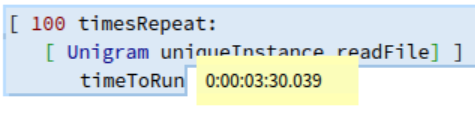
\includegraphics[width=0.7\linewidth]{images/unigramTimeToRunSlow.png}
    \caption{It takes more than 3 minutes to read the results from file on repeat 100 times}
    \label{fig:sorterSlow}
\end{figure}

The approach to improve the time efficiency was to set a certain threshold for the number of occurences, and to cut off all the tokens with frequencies below it. I put the threshold equal to 10, meaning if the token occured less than 10 times throughout the whole history, it was irrelevant enough to be discarded. This way, I was able to cut off most of the miscellaneous, rarely encountered tokens, and shortened the dataset from 150k to just 16k entries. This made the frequencies lookup during completion sorting very fast and, as a result, it was now possible to type and use completion information without any delays (see the improvement in Figure \ref{fig:sorterFast}).

\begin{figure}[H]
    \centering
    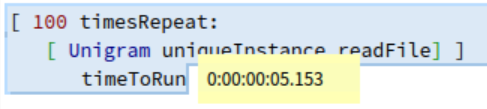
\includegraphics[width=0.7\linewidth]{images/unigramTimeToRunFast.png}
    \caption{After the cut off, it takes only 5 seconds to run it 100 times}
    \label{fig:sorterFast}
\end{figure}

The one-time tokens, such as custom strings and comments, did not make a big difference during the implementation of the unigram sorting strategy, however when I moved on to implementing the bigram sorter, the model became "too heavy" due to many combinations of such tokens, and needed to be additionally reduced.

The solution was to go back to the data processing step and replace those "one-time" tokens with placeholders. In particular, I added placeholders for strings, comments, symbols, characters, arrays and numbers (such as all strings being written as <str> and all numbers as <num>). This greatly reduced both the number of total tokens and the subsequent ngram sequences, which helped both the bigram and the unigram model, as well as the lookup speed (for example, for the unigram model even without the threshold cut-off, with the placeholder replacement the number of tokens was reduced from 150k to just 85k, and for the bigram model the vocabulary size also got reduced in half).

\section{Using the N-gram Sorters}
\label{sec:ProposedSolution-Usage}
It is worth noting that both the n-gram sorters can actually be used in the Pharo IDE by loading the CompletionSorting library\footnote{\url{https://github.com/myroslavarm/CompletionSorting}}, which contains the implementation of this experiment. The unigram-based sorter is available as the FrequencyCompletionSorter, and the bigram-based as the BigramCompltionSorter -- they can be used by enabling the respective sorting option in the Settings (Figure \ref{fig:settings}, below).

The unigram sorter is quite fast and accurate (we go over the quality of the performance in Chapter \ref{chap:Evaluation}). However, the bigram sorter is too slow for comfortable usage, and re-engineering the implementation to be faster is left for future work.

\begin{figure}[H]
    \centering
    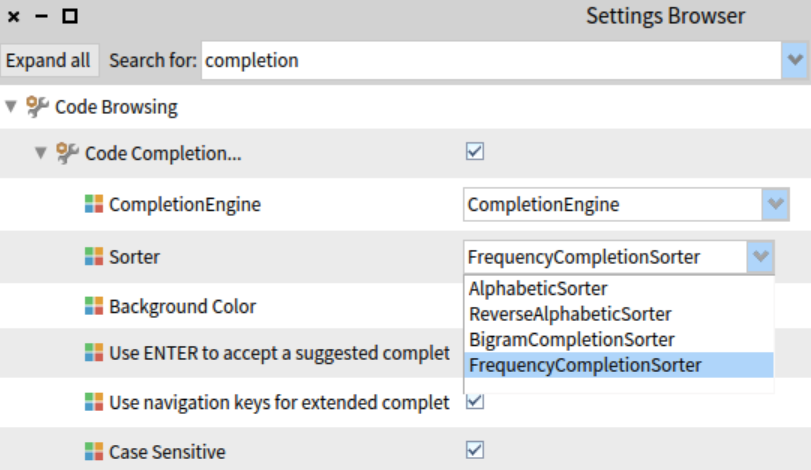
\includegraphics[width=0.9\linewidth]{images/settings.png}
    \caption{The Settings window in the Pharo IDE}
    \label{fig:settings}
\end{figure}

\section{Summary}
\label{sec:ProposedSolution-Summary}
\begin{itemize}
    \item The data used to train the models came from 50 projects implemented in Pharo; in the dataset the source code was already split into tokens and token types. In the data, delimiters and non-alphabetic tokens, as well as comments, were all considered to be separate tokens.
    \item For unigram sorting, individual token frequencies were extracted and the sorting of completions was based on those frequencies.
    \item For bigram sorting, completion candidates were added to the previous token to form sequences of bigrams, whose probability was later calculated and recorded to file; the sorting was based on the sequence probability but it was only applied to individually displayed completion candidates.
    \item Different approaches were taken to reduce the sizes of models and speed up lookup and sorting time; among them: cleaning up tokens with occurences below a certain threshold, and replacing "one-time" tokens (such as specific strings, numbers, and so on) with general placeholders (such as <str>, <num>).
    \item In the process of working on the bigram sorting strategy, the NgramModel Pharo library that was used for this approach was addiitionally extended with new functionality, such as reading/writing to file and reducing the number of sequences with counts below a certain threshold.
    \item Finally, both sorting strategies can be enabled to be used in the Pharo IDE, however the bigram sorter remains too slow for comfortable day-to-day usage.
\end{itemize}